\documentclass[12pt, a4paper]{report}
\usepackage{ctex} % 中文的宏包
\usepackage{indentfirst}
\usepackage{graphicx} % 插入圖片的宏包
\usepackage{float} % 設置圖片浮動位置的宏包
\usepackage{subfigure} % 插入多圖時用子圖顯示宏包
\usepackage{listings} % 代碼塊宏包
\usepackage{color} % 代碼高亮
\usepackage[colorlinks,linkcolor=blue]{hyperref} % URL 包
\usepackage[pdf]{graphviz}

\definecolor{dkgreen}{rgb}{0,0.6,0}
\definecolor{gray}{rgb}{0.5,0.5,0.5}
\definecolor{mauve}{rgb}{0.58,0,0.82}

\lstset{ %
    %language=Octave,                % the language of the code
    basicstyle=\scriptsize\Hack,           % the size of the fonts that are used for the code
    numbers=none,                   % where to put the line-numbers
    numberstyle=\tiny\color{gray},  % the style that is used for the line-numbers
    stepnumber=2,                   % the step between two line-numbers. If it's 1, each line 
                                    % will be numbered
    numbersep=3pt,                  % how far the line-numbers are from the code
    backgroundcolor=\color{white},      % choose the background color. You must add \usepackage{color}
    showspaces=false,               % show spaces adding particular underscores
    showstringspaces=false,         % underline spaces within strings
    showtabs=false,                 % show tabs within strings adding particular underscores
    frame=single,                   % adds a frame around the code
    rulecolor=\color{black},        % if not set, the frame-color may be changed on line-breaks within not-black text (e.g. commens (green here))
    tabsize=2,                      % sets default tabsize to 2 spaces
    captionpos=b,                   % sets the caption-position to bottom
    breaklines=true,                % sets automatic line breaking
    breakatwhitespace=false,        % sets if automatic breaks should only happen at whitespace
    title=\lstname,                   % show the filename of files included with \lstinputlisting;
                                    % also try caption instead of title
    keywordstyle=\color{blue},          % keyword style
    commentstyle=\color{dkgreen},       % comment style
    stringstyle=\color{mauve},         % string literal style
    escapeinside={\%*}{*},            % if you want to add LaTeX within your code
    morekeywords={*,...}               % if you want to add more keywords to the set
}
\setCJKmainfont{Noto Serif CJK TC} % 主要字體 Noto Serif
\newfontfamily\Hack{Hack} % 代碼字體
\author{軟件 1804 8209180438 黃柏曛}
\date{\today}
\title{數據庫系統 SSD7 實驗報告}
\begin{document}

\maketitle

\tableofcontents

\part{實驗一、數據庫與表的基本操作}

\section{實驗目的}

\begin{itemize}
    \item 熟练掌握一种DBMS的使用方法,完成数据库的创建、删除和连接;数据表的建立、删除;表结构的修改。
    \item 加深对表的实体完整性、参照完整性和用户自定义完整性的理解。
\end{itemize}

\section{實驗內容}

以下实验中,使用学生-课程数据库,它描述了学生的基本信息、课程的基本信息及学生选修课程的信息。用SQL语句分别完成。

\subsection{创建学生-课程数据库}

{数据文件名为 $student\_data$、大小10M,日志文件名为 $student\_log$、大小5M的新数据库,该数据库名为 $student\_xxxxxx$,xxxxxx表示班级学号。1801班12号,数据库名为 $student\_180112$}。

\subsection{創建 Table}

\begin{figure}[H] % H 為當前位置,!htb 為忽略美學標準,htbp 為浮動圖片
    \centering % 圖片居中
    \subfigure[创建学生关系表S]{
    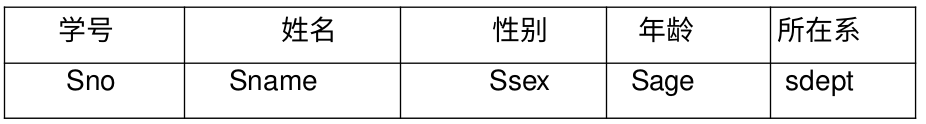
\includegraphics[width=1\textwidth]{ex1-1.png}} % 插入圖片,[] 為圖片大小,{} 是圖片文件
    \subfigure[创建课程关系表C]{
    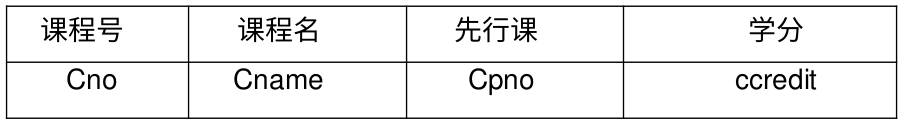
\includegraphics[width=0.8\textwidth]{ex1-2.png}}
    \subfigure[创建学生-课程表SC]{
    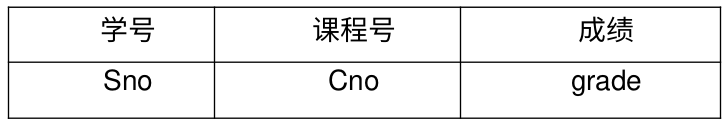
\includegraphics[width=0.75\textwidth]{ex1-3.png}}
\end{figure}

\begin{itemize}
    \item 将以上创建表S、C、SC的SQL命令以 .SQL文件的形式保存在磁盘上。在表中加入至少4个元组,第一个为本人信息。
    \item 在表S上增加“出生日期”与“身高”属性列。
    \item 删除表S的“身高” 属性列。
    \item 备份数据库,再还原。
\end{itemize}

\section{實驗方法與實驗步驟}

\begin{itemize}
    \item 创建数据库或连接已建立的数据库。
    \item 在当前数据库上建立新表。
    \item 定义表的结构。
    \item 修改表的结构。
\end{itemize}

\section{實驗結果}

\subsection{在 ArchLinux 上配置好 MySQL}

\begin{lstlisting}[language=Octave]
    $ sudo pacman -S mariadb # 安裝 mariadb
    $ chattr +C /var/lib/mysql # disabling Copy-on-Write,因為我的文件系統是 Btrfs
    $ systemctl enable mariadb # 啟用
    $ systemctl start mariadb # 執行
    $ sudo mysql -u root -p # 以 root 身份進行
\end{lstlisting}

{可以自己設定一些密碼或是新增使用者}

\subsection{創建 student\_data database}

\begin{figure}[H] % H 為當前位置,!htb 為忽略美學標準,htbp 為浮動圖片
    \centering % 圖片居中
    \subfigure[創建 database]{
    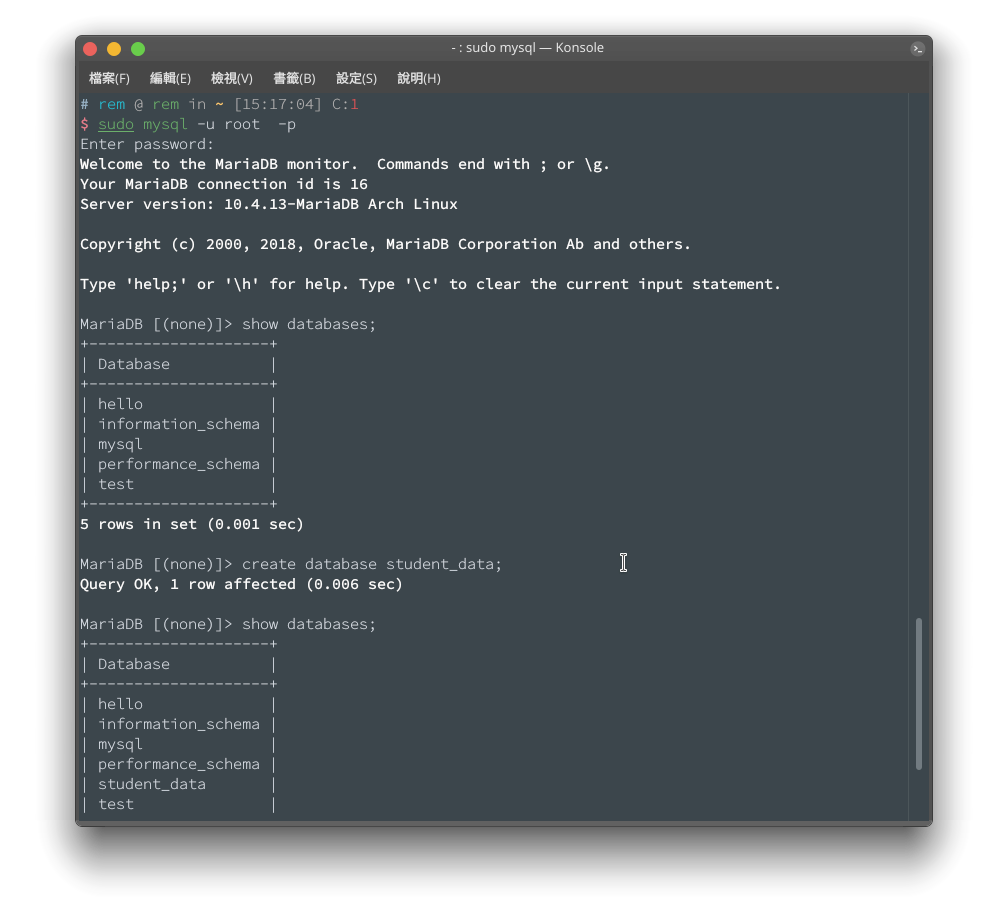
\includegraphics[width=1\textwidth]{ex1-4.png}}
\end{figure}

\subsection{將 Table 創建出來}

{至少每個 Table 填入四筆數據}

\begin{figure}[H] % H 為當前位置,!htb 為忽略美學標準,htbp 為浮動圖片
    \centering % 圖片居中
    \subfigure[創建 Table S]{
    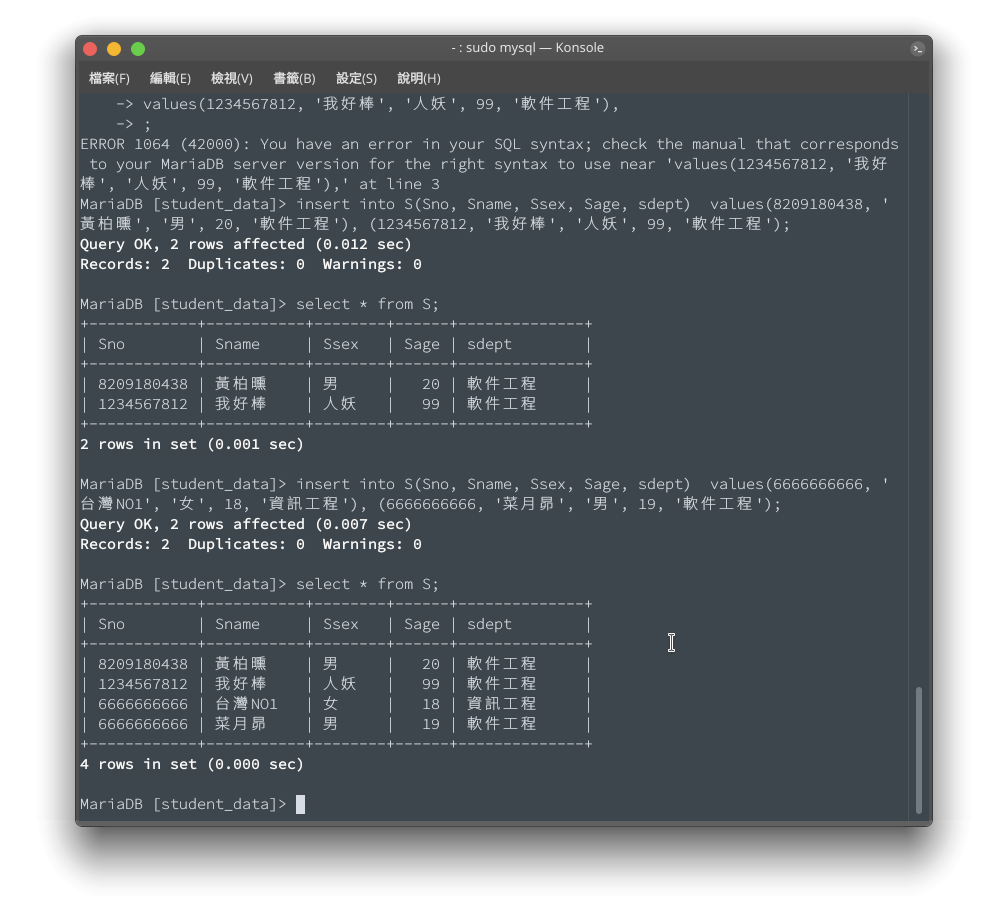
\includegraphics[width=1\textwidth]{ex1-5.png}}
\end{figure}

\begin{figure}[H] % H 為當前位置,!htb 為忽略美學標準,htbp 為浮動圖片
    \centering % 圖片居中
    \subfigure[創建 Table C]{
    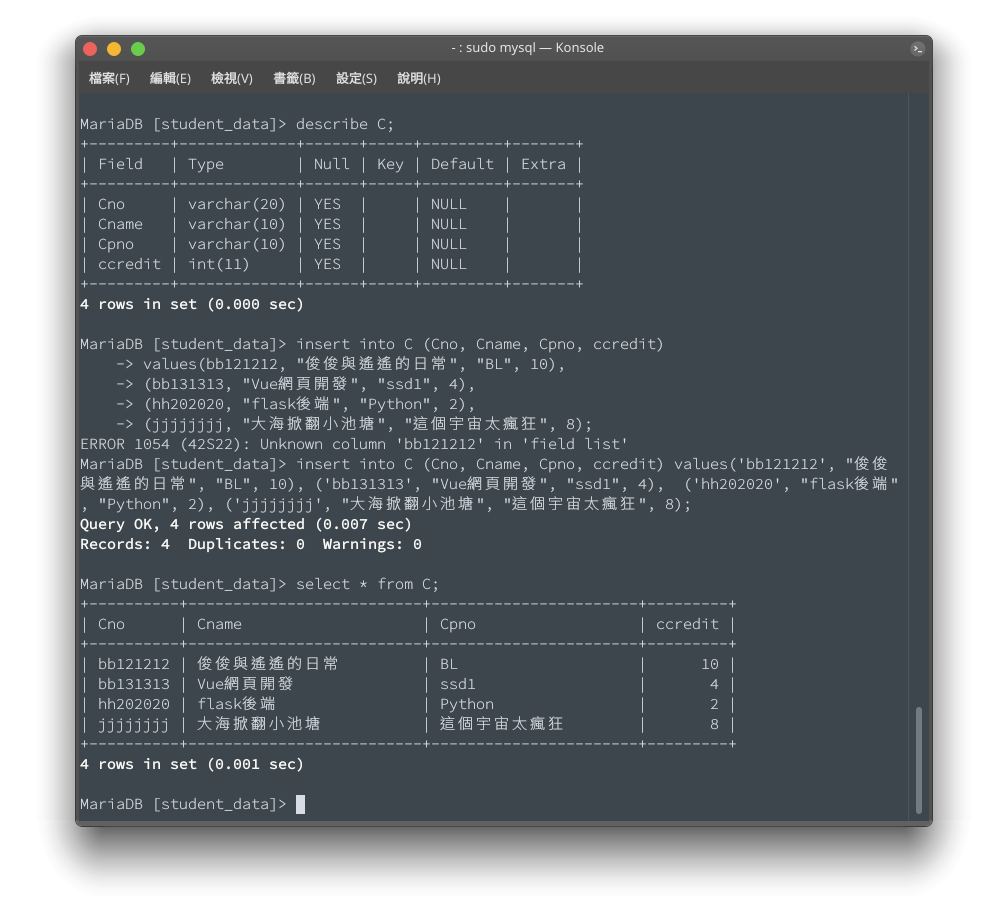
\includegraphics[width=1\textwidth]{ex1-6.png}}
\end{figure}

\begin{figure}[H] % H 為當前位置,!htb 為忽略美學標準,htbp 為浮動圖片
    \centering % 圖片居中
    \subfigure[創建 Table SC]{
    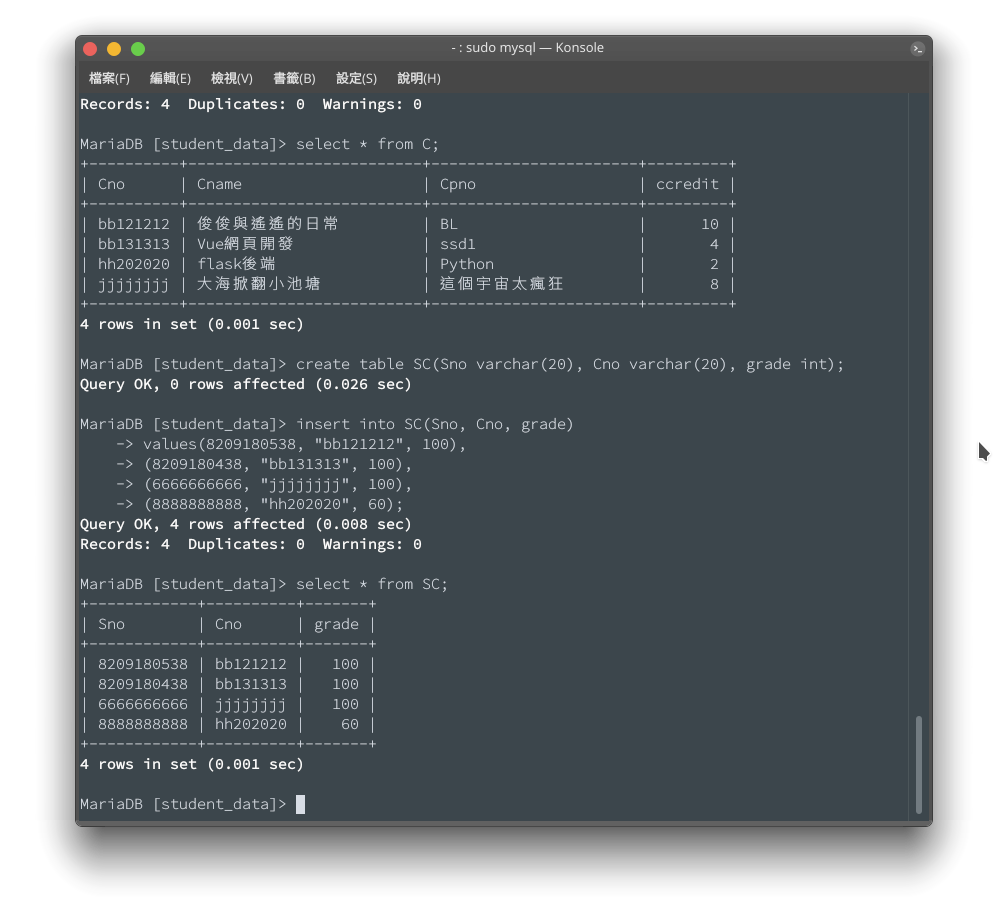
\includegraphics[width=1\textwidth]{ex1-7.png}}
\end{figure}

\subsection{新增屬性列與刪除屬性列}

在 S Table 新增 SBirthday(生日)與 SHeight(身高)。

\begin{figure}[H] % H 為當前位置,!htb 為忽略美學標準,htbp 為浮動圖片
    \centering % 圖片居中
    \subfigure[Table S 添加列]{
    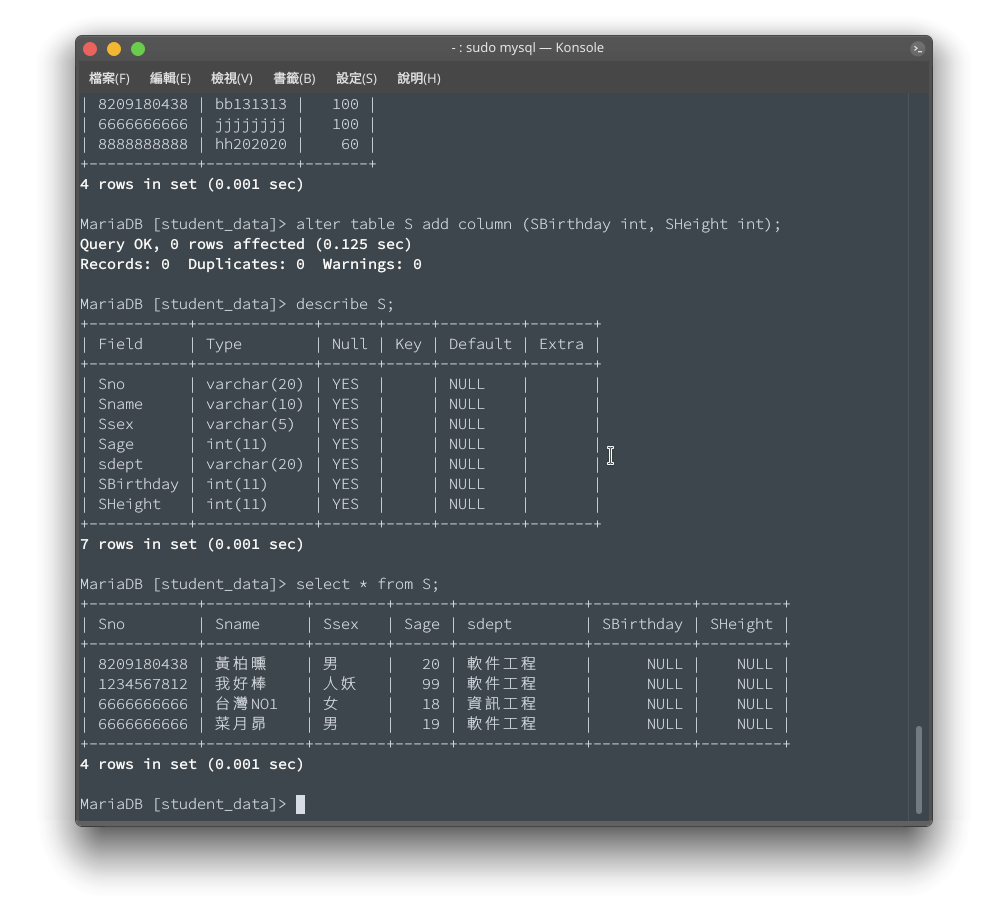
\includegraphics[width=1\textwidth]{ex1-8.png}}
\end{figure}

刪除 S Table 中的 SHeight(身高)。

\begin{figure}[H] % H 為當前位置,!htb 為忽略美學標準,htbp 為浮動圖片
    \centering % 圖片居中
    \subfigure[Table S 刪除列]{
    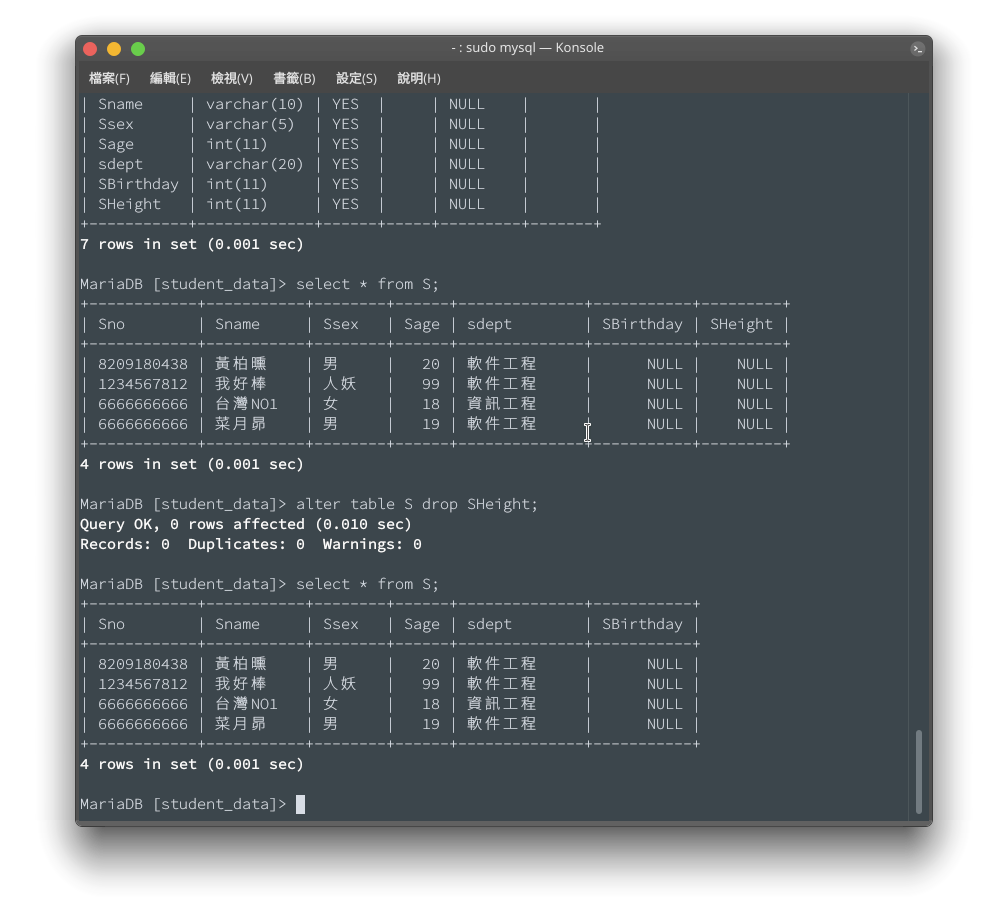
\includegraphics[width=1\textwidth]{ex1-9.png}}
\end{figure}

\subsection{SQL 的備份與還原}

匯出 mySQL 文件

\begin{figure}[H] % H 為當前位置,!htb 為忽略美學標準,htbp 為浮動圖片
    \centering % 圖片居中
    \subfigure[匯出 student\_data.sql 文件]{
    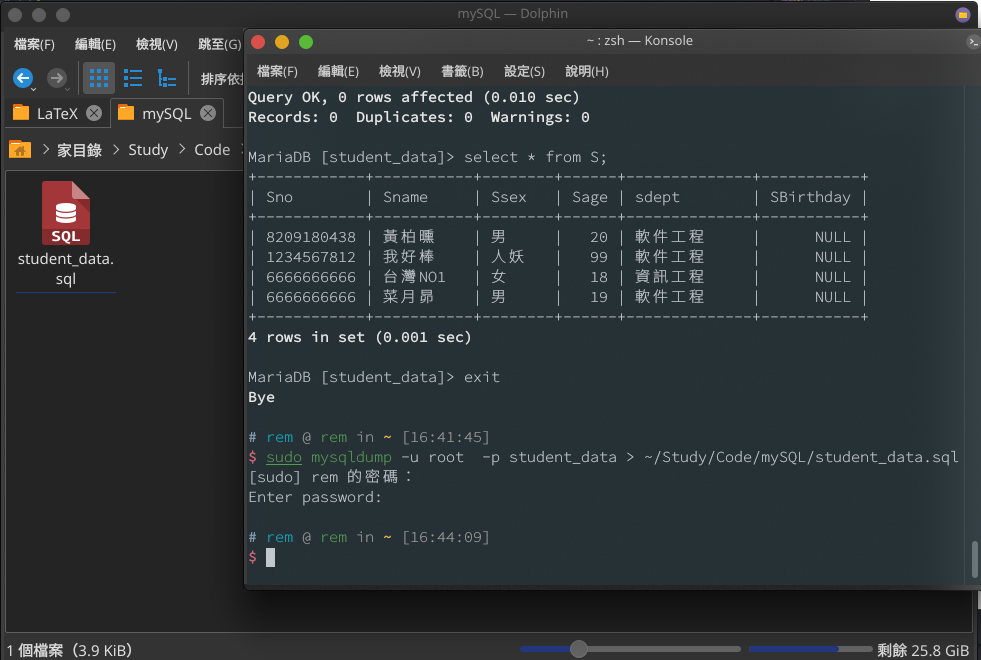
\includegraphics[width=1\textwidth]{ex1-10.png}}
\end{figure}

匯入 mySQL 文件

\begin{figure}[H] % H 為當前位置,!htb 為忽略美學標準,htbp 為浮動圖片
    \centering % 圖片居中
    \subfigure[匯入 student\_data.sql 文件]{
    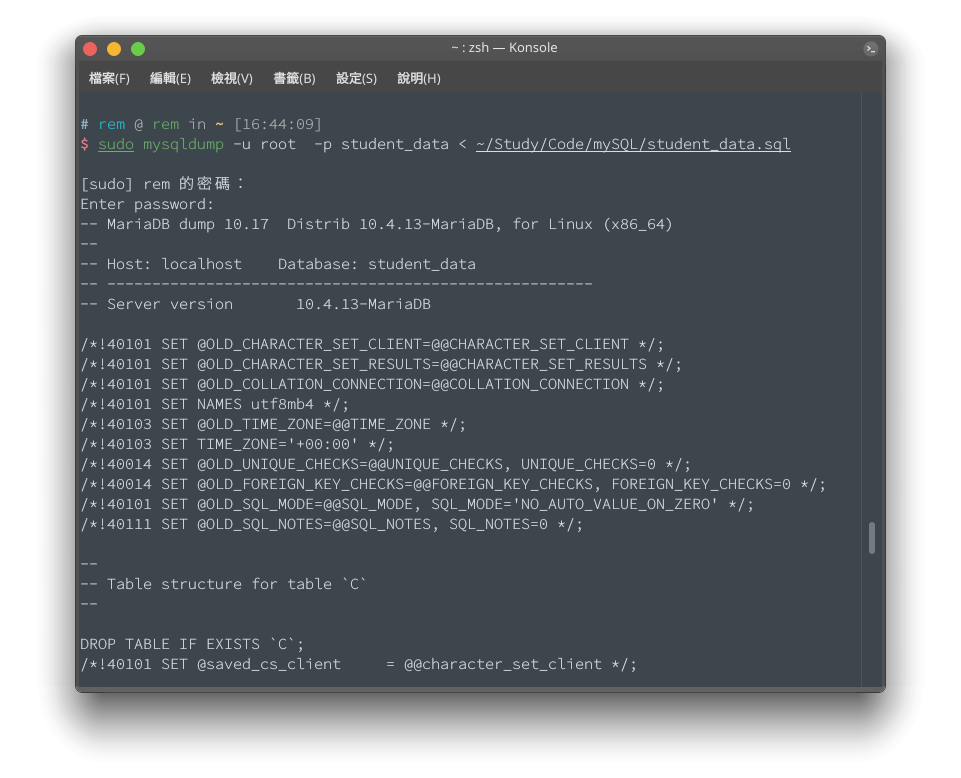
\includegraphics[width=1\textwidth]{ex1-11.png}}
\end{figure}

\begin{figure}[H] % H 為當前位置,!htb 為忽略美學標準,htbp 為浮動圖片
    \centering % 圖片居中
    \subfigure[student\_data 已被還原]{
    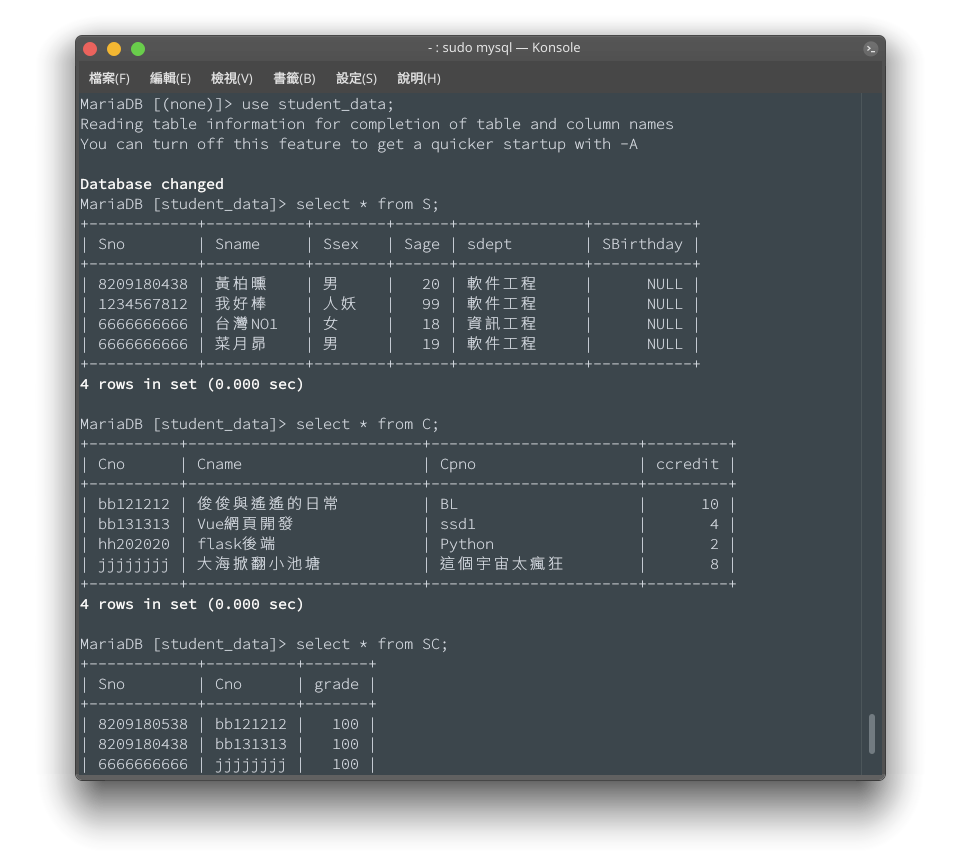
\includegraphics[width=1\textwidth]{ex1-12.png}}
\end{figure}

\section{實驗小結}

本次實驗讓我們學習基本的數據庫操作,讓我們了解數據庫的基本指令,我也在這次實驗學會了怎麼使用數據庫。有時我打指令會忘記在每行指令後面添加分號,造成要重打一次,不過這樣是讓我養成習慣。

\part{實驗二、數據庫查詢與更新}

\section{實驗目的}

\begin{itemize}
    \item 熟悉和掌握对数据表中数据的查询操作和SQL命令的使用,学会灵活熟练的使用SQL 语句的各种形式,加深理解关系运算的各种操作(尤其是关系的选择,投影,连接和除运算);
    \item 熟悉和掌握数据表中数据的插入、修改、删除操作和命令的使用(熟悉使用UPDATE/INSERT/DELETE语句进行表操作);加深理解表的定义对数据更新的作用。
\end{itemize}

\section{實驗內容}



\section{實驗方法與實驗步驟}

\section{實驗結果}

\section{實驗小結}

\part{實驗一、數據庫與表的基本操作}

\section{實驗目的}



\section{實驗內容}

\section{實驗方法與實驗步驟}

\section{實驗結果}

\section{實驗小結}

\part{實驗一、數據庫與表的基本操作}

\section{實驗目的}



\section{實驗內容}

\section{實驗方法與實驗步驟}

\section{實驗結果}

\section{實驗小結}

\part{實驗一、數據庫與表的基本操作}

\section{實驗目的}



\section{實驗內容}

\section{實驗方法與實驗步驟}

\section{實驗結果}

\section{實驗小結}

\end{document}